\documentclass{unicam_thesis}

\usepackage[font=footnotesize,labelfont=bf]{caption}
\usepackage{savesym}
\savesymbol{framed} % Fix per Framed
\usepackage[newfloat]{minted}
\restoresymbol{TXF}{framed}  % Fix per Framed
\usepackage{csquotes} 
\usepackage{caption}
\usepackage{xpatch}
\usepackage[square, numbers]{natbib}
\usepackage[svgnames]{xcolor}

\author{Diego Pasquali}
\advisor{Prof. Luca Tesei}
\academicyear{2016/2017}
\matricola{093341}

\university{Universit\`a degli Studi di Camerino}
\school{Scienze e Tecnologie}
\course{Laurea in Informatica (Classe L-31)}

\title{La gestione del flusso dei dati nel front-end di applicazioni web complesse}

% Bibliografia
\renewcommand*{\bibfont}{\raggedright}
\renewcommand{\UrlFont}{\small\tt}

% Minted setup
\captionsetup[listing]{position=bottom,skip=-7pt}
\SetupFloatingEnvironment{listing}{name=Codice}
\usemintedstyle{algol_nu}
\setminted{fontsize=\footnotesize, baselinestretch=1.3, bgcolor=WhiteSmoke} 

% Rimuove il box rosso attorno agli errori di Minted
\makeatletter
\AtBeginEnvironment{minted}{\dontdofcolorbox}
\def\dontdofcolorbox{\renewcommand\fcolorbox[4][]{##4}}
\xpatchcmd{\inputminted}{\minted@fvset}{\minted@fvset\dontdofcolorbox}{}{}
\makeatother

\begin{document}
    \maketitle

    \chapter*{Abstract}

In questa tesi viene trattata la problematica relativa alla gestione del flusso dei dati e degli eventi che modificano direttamente o indirettamente l'interfaccia di una applicazione web moderna. Avere un adeguato controllo su questo flusso è di primaria importanza al fine di ottenere un servizio il cui codice sia chiaro e con uno stato che cambi in maniera comprensibile e deterministica, dove sia semplice riprodurre eventuali errori ed aggiungere nuovi elementi.

In questo documento verranno messe a confronto architetture innovative come \textit{Flux} e \textit{Redux} che implementano un flusso di dati unidirezionale, con altre più datate come \textit{MVC} e derivate che invece scelgono un flusso bidirezionale. 
L'analisi sarà approfondita con degli esempi di codice per ognuno di questi paradigmi in modo da effettuare una dimostrazione pratica delle loro principali differenze.
    
    \tableofcontents

    \chapter{Introduzione}
Il \textit{Flusso dei dati} nel front-end di una applicazione web rappresenta tutti gli input e gli eventi che si muovono attraverso i suoi vari livelli logici. Per fare un esempio semplicistico della questione, il banale cliccare su un bottone in un qualsiasi servizio online moderno, fa scaturire un evento che porta con sé dei dati che andranno ad apportare dei cambiamenti nello stato dell'applicazione. Ciascun elemento dell'interfaccia deve successivamente tener conto di questo cambiamento e modificarsi di conseguenza se necessario. Più questo flusso di dati è intenso e disorganizzato, più diventa complicato gestire i cambi di stato e la loro propagazione attraverso tutti i vari componenti.

Un'interfaccia utente quindi mette a disposizione dell'utilizzatore una immensa quantità di interazioni, sia volontarie che involontarie, che cambiano in continuazione lo stato dell'applicazione e che devono essere opportunamente gestite e sincronizzate. La struttura del codice diventa quindi prioritaria al fine di ottenere un prodotto che sia soddisfacente a livello di prestazioni e che riesca a mantenere un adeguato livello di scalabilità.

L'obbietto principale di questa tesi consiste nel fornire una presentazione delle varie architetture e dei vari approcci utilizzati attualmente per risolvere il problema della gestione del flusso di dati in applicazioni web con una codebase solitamente grande e complessa, comparando i loro relativi vantaggi e svantaggi. Verrà effettuata un'analisi approfondita del paradigma \textit{MVC} (Model - View - Controller) lato front-end, spiegando le grosse differenze che si vengono a creare rispetto al suo utilizzo lato back-end e alla sua scarsa scalabilità derivata dall'uso di un flusso di dati bidirezionale tra Model e View. Verranno poi discusse le architetture di \textit{Flux} e di \textit{Redux} che implementano un flusso di dati unidirezionale per ovviare ai problemi del paradigma MVC.
L'analisi coprirà le differenze di implementazione delle due librerie, di come Flux si basi su una struttura complessa ma estremamente funzionale oltre che versatile, e di come Redux la semplifichi attraverso pattern della programmazione funzionale per ottenere lo stesso livello di scalabilità con una semplicità decisamente maggiore.

\section{Background}
La gestione del flusso dei dati all'interno di una applicazione web è un argomento molto discusso dopo l'avvento di tecnologie front-end sempre più complesse e potenti come \textit{React} o \textit{Angular} ma sopratutto con la crescita smisurata della complessità dei servizi online. La causa di ciò è la necessità di avere un codice che sia il più possibile scalabile ed il più facilmente testabile a prescindere dal numero di features che verranno successivamente aggiunte. 

\begin{figure}[h]
\centering 
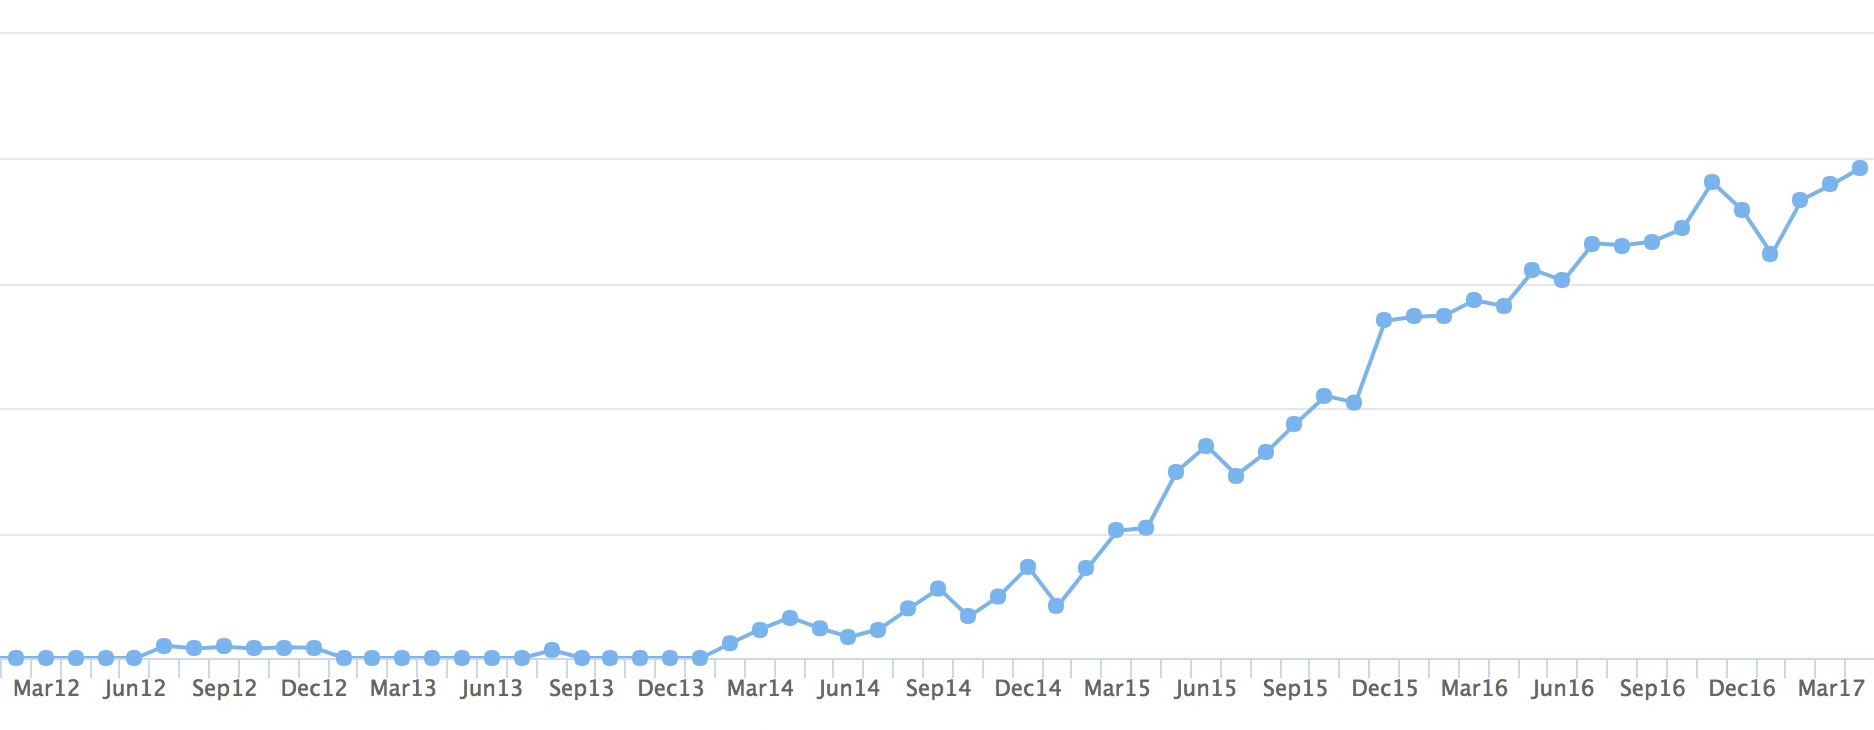
\includegraphics[width=12.7cm]{./images/reactPopularity}
\caption{Grafico della popolarità di React (generato da \href{https://www.hntrends.com/}{hntrends.com}).}
\end{figure}

\noindent
Codebase vaste come potrebbero essere quelle di Facebook, Twitter o YouTube necessitano di una architettura di fondo che sia altamente chiara e comprensibile per evitare confusione tra i vari servizi.
Come vedremo successivamente, architetture datate come l'MVC pur essendo molto efficienti lato back-end non rendono allo stesso modo lato front-end, dove c'è una quantità maggiore di azioni che l'utente può intraprendere e che possono avere ripercussioni differenti su più componenti diversi all'interno di una View.
In questo documento verranno discusse le alternative attualmente più gettonate come quella a flusso unidirezionale, implementata in prima battuta da Flux e successivamente ottimizzata da Redux.

\section{Lo stato dell'arte}
Possiamo paragonare la creazione della prima applicazione web con la messa online del primo sito da parte di Tim Berners-Lee nel 1991 dal Cern di Ginevra \cite{HuffingtonpostFirstWebsite}. Stiamo tuttavia parlando di una applicazione statica costruita solamente in HTML dove gli unici input dell'utente erano limitati al navigare i documenti. Più avanti con l'evoluzione di HTML si iniziarono a vedere i primi elementi interattivi come bottoni e campi di testo. Tuttavia la svolta vera e propria avvenne il 5 maggio del 1995 con l'avvento di Javascript \cite{W3cJavascriptHistory}, il linguaggio di scripting che portò un primo accenno di dinamicità all'interno delle pagine web e che anche adesso è alla base di tutte le tecnologie front-end più nuove e potenti. Da qui in poi l'evoluzione andò avanti in maniera esponenziale partendo da un utilizzo banale del linguaggio fino a giungere alla situazione attuale con framework ed architetture complesse.

\subsection{Single-page application}
Andando avanti con gli anni si sono tentati diversi approcci per la creazione di applicazioni web. Un problema fondamentale è stato quello di dove posizionare la logica del servizio che fino a quel momento è stata sempre considerata come una parte del server specialmente per la mancanza di tecnologie adeguate lato client.

\begin{figure}[h]
\centering
\includegraphics[width=10cm]{./images/noSPA}
\caption{Esempio di una applicazione con la logica nel server.}
\end{figure}

Con la maturazione degli strumenti client-side si è aperta una porta ad un nuovo tipo di applicazioni: le \textit{Single-page application} (SPA). Una Single-page application è una applicazione web contenuta in una sola pagina e che sviluppa tutta la sua logica nel client.

Non è da poco che questo tipo di applicazioni hanno preso piede, tuttavia intorno agli anni 2000 non era Javascript la prima scelta come linguaggio di programmazione ma Flash e Java Applets. Solo più avanti è riuscito a diventare competitivo abbastanza da deprecare entrambi i suoi predecessori per diversi motivi \cite{mikowski2013single}:

\begin{itemize}
    \item \textbf{Velocità di esecuzione} Javascript non ha bisogno di alcun ambiente esterno per essere eseguito consentendo di eliminare un livello di complessità all'applicazione.
    \item \textbf{Nessuna dipendenza esterna} Gli utenti non hanno bisogno di scaricare nessuna dipendenza esterna e quindi nessun plugin per eseguire il servizio.
    \item \textbf{Controllo sulla pagina web} Javascript ha pieno controllo sulla pagina web dove viene eseguito in quanto è tutt'uno con essa. Al contrario, Flash e Java, vengono inseriti in maniera “embedded" nella pagina e non hanno la possibilità di interagire con essa in maniera diretta causando un'esperienza meno fluida ed interattiva per l'utente.
\end{itemize}

\begin{figure}[h]
\centering
\includegraphics[width=10cm]{./images/yesSPA} 
\caption{Esempio di una applicazione SPA.}
\end{figure}

\noindent
La problematica della gestione del flusso dei dati è diventata estremamente rilevante con la comparsa delle SPA in Javascript. Nel loro stadio iniziale queste non erano costruite sopra una struttura ben definita e la gestione del flusso dei dati avveniva in maniera disordinata gestendo ogni azione dell'utente in maniera diretta.
Andando avanti con il tempo e con l'aumentare della complessità di queste applicazioni, si è sentito il bisogno di creare un'architettura ben definita che aiutasse a gestire in maniera più consistente lo stato del servizio e tutti i suoi eventuali cambiamenti.

\subsection{I primi framework basati su MVC}
La necessità di avere struttura più solida lato front-end, specialmente per applicazioni più esigenti, ha portato alla nascita dei primi framework basati sull'architettura MVC.

\blockquote{Single page apps are distinguished by their ability to redraw any part of the UI without requiring a server roundtrip to retrieve HTML. This is achieved by separating the data from the presentation of data by having a model layer that handles data and a view layer that reads from the models. \cite{MixuSinglePageWebApp}}

\noindent Nel modello MVC per front-end (e come anche in quello back-end), che riprenderemo in dettaglio più avanti nel documento, abbiamo una netta distinzione tra i dati (Model), la presentazione di quest'ultimi (View) e la logica che funge da tramite (Controller), incaricata di gestire le richieste degli utenti e gli eventi che accadono all'interno dell'applicazione fornendo i dati necessari alla costruzione della View. Questo ci permette di avere un controllo maggiore sullo stato globale e di ogni singolo componente dell'interfaccia oltre ad un codice più robusto e facile da modificare nel tempo \cite{ParrOnTheMVC}.

Javascript ha a disposizione un numero considerevolmente alto di framework MVC. Uno dei più famosi è sicuramente \textit{AngularJS} (parliamo della versione 1) \cite{AngularOfficialDocumentation}, mantenuto da Google e dalla vasta community formatasi intorno.
L'architettura MVC lato front-end non è considerata però ottimale. Col passare del tempo si sono venute a creare delle strutture derivate da questa che tendono a sviluppare la gestione dell'interfaccia utente in maniera differente, con i propri vantaggi e svantaggi. Una di queste è MVP (Model - View - Presenter) utilizzata da \textit{Backbone.js}\footnote{http://backbonejs.org}. In questa il Presenter, che sostituisce il Controller, ha una responsabilità minore di quest'ultimo e si occupa solamente di passare dati alla View la quale deciderà cosa e come mostrare. Un'altra architettura derivata da MVC è MVVM (Model - View - ViewModel), utilizzata da framework come \textit{Knockout}\footnote{http://knockoutjs.com}, in cui il ViewModel si occupa di mantenere i dati del Model (che sono grezzi) nella forma richiesta dalla View, ed espone a quest'ultima metodi e funzioni per la gestione dello stato dell'applicazione \cite{ChauhanFrontendArchitectures}.

Ancora una volta tuttavia ci troviamo di fronte ad un muro, dove le architetture venutesi a creare sono tante ma tutte derivate da MVC traendone i difetti. Il problema più grande di questo paradigma è la comunicazione bidirezionale: una View, tramite il Controller, modifica diversi Model i quali a loro volta aggiornano le relative View. Tenendo presente che stiamo parlando di applicazioni complesse e quindi con un grande numero di componenti, questo genera un effetto cascata di modifiche tra i vari Model e View causando una codebase molto difficile da gestire ed analizzare. 

Per la prima volta a questo punto si inizia a discutere di flusso di dati in maniera attiva e diretta riconoscendolo come difetto principale del modello MVC e trovando in React la libreria perfetta per risolverlo \cite{SalihefendicFluxVsMVC}.

\subsection{Framework ed architetture a flusso unidirezionale}
Un ulteriore passo avanti nella storia delle applicazioni web è stata React\footnote{https://facebook.github.io/react}, libreria per la creazione di interfacce utente sviluppata da Facebook che si basa su diverse tecnologie all'avanguardia e che permette grazie alla sua versatilità di strutturare architetture più complesse ed efficienti.
React è una libreria e non un framework, ciò significa che il suo lavoro è solamente quello di creare interfacce utente \cite{BunaReactIsTheNewFrontend}. Non è quindi una soluzione finale ma un componente fondamentale che unito ad altri ci permette di scrivere applicazioni web in maniera molto più dinamica.

Per sfruttare al massimo una libreria come React, Facebook mette anche a disposizione una struttura che sembra risolvere il problema relativo alla comunicazione bidirezionale riscontrato nel paradigma MVC. \textit{Flux}\footnote{https://facebook.github.io/flux} è un'architettura complessa per la costruzione di interfacce utente che si basa su un flusso di dati unidirezionale facilmente gestibile ed altamente scalabile. In Flux una View non modifica mai in maniera diretta lo stato di una applicazione, bensì propaga azioni che vengono gestite da un \textit{Dispatcher} e che hanno delle ripercussioni sul Model di questo paradigma che si chiama \textit{Store}. Infine, quest'ultimo si occupa di propagare a sua volta un evento a tutti i componenti delle View che permette loro di aggiornarsi di conseguenza. Questo tipo di approccio di permette di avere un flusso di dati facilmente analizzabile in quanto sappiamo esattamente dove arrivano in input e dove escono in output i dati di ogni singolo strato dell'architettura ma sopratutto ci permette di gestire in maniera chiara e pulita la sincronizzazione tra stato ed ogni singolo componente dell'interfaccia utente.

\subsection{Un approccio funzionale al flusso unidirezionale: Redux}
Flux riesce a risolvere a pieno tutti i problemi fino ad ora descritti causati dalla comunicazione bidirezionale delle architetture MVC e derivate. Tuttavia la complessità di tale paradigma si fa sentire già da subito sia per il gran numero di passaggi che un'azione deve effettuare prima di essere effettivamente eseguita, sia per la difficoltà nell'implementazione anche in applicazioni di medio-piccole dimensioni.

Un'alternativa che si basa sempre su Flux è \textit{Redux}\footnote{http://redux.js.org}, una libreria scritta da Dan Abramov e Andrew Clark che si identifica come semplice “Gestore dello stato" di una applicazione \cite{ReduxOfficialDocumentation}. Redux riesce a semplificare l'architettura di Flux utilizzando dei pattern della programmazione funzionale come la composizione e l'immutabilità per ottenere una struttura a flusso unidirezionale eliminando il Dispatcher e altre complessità \cite{AbramovOnReduxVsFlux}.

Vedremo nei prossimi capitoli come sia semplice ed elegante gestire il flusso dei dati e lo stato di un'applicazione che utilizza Redux e React, e come questi risolvono in dettaglio le principali problematiche delle architetture descritte precedentemente.
    \chapter{Strumenti}
Per analizzare le varie architetture presentate dobbiamo prima fare un discorso sugli strumenti utilizzati per costruire una applicazione web e che useremo per gli esempi di codice dei capitoli successivi.

\section{ECMAScript 2015}
Anche conosciuto come \textit{ECMAScript6}, è una standardizzazione del linguaggio Javascript creata da Ecma International. Questa versione in particolare mette a disposizione features molto utili per scrivere codice funzionale. Possiamo classificare ECMAScript come un linguaggio a sé e differente da Javascript, che in principio doveva essere utilizzato solamente come linguaggio di scripting lato web, ma che ora viene utilizzato come vero e proprio linguaggio di programmazione su ambienti e scale differenti \cite{ECMAScriptDocumentation}.
 
In ambito web non tutte le features di ES6 sono disponibili, per questo si utilizzano strumenti come \textit{Babel} o \textit{Webpack} che hanno la funzione di \textit{transpiler}, ossia di compilare codice sorgente da ECMAScript6 a ECMAScript5 che è supportato dalla stragrande maggioranza dei browser.

Le funzionalità introdotte da ECMAScript6 sono molte, tuttavia qui parleremo solo di quelle che risulteranno propedeutiche per capire i pezzi di codice nei capitoli successivi.

\subsection{Let e Const}
Una delle features introdotte, che probabilmente è anche una delle più incisive, riguarda l'assegnazione delle variabili. In ES5 la dichiarazione avveniva tramite la keyword \textit{var} ed il loro scope era relativo alla funzione direttamente loro superiore (codice \ref{exampleVarES5}).
 
\begin{listing}[ht]
\inputminted{Javascript}{sources/exampleVarES5.js}
\caption{Esempio della dichiarazione di una variabile con \textit{var}.}
\label{exampleVarES5}
\end{listing}

\noindent
In ES6 a questa si aggiungono anche \text{let} e \textit{const} il cui scope è relativo al blocco in cui sono posizionate (e non alla funzione, come in \textit{var}). La prima non ha nulla di particolare oltre ciò che abbiamo già detto, la seconda invece dichiara variabili costanti, ossia il cui valore non può mutare (codice \ref{exampleLetConstES6}).

\begin{listing}[ht]
\inputminted{Javascript}{sources/exampleLetConstES6.js}
\caption{Esempio della dichiarazione di variabili con \textit{let} e \textit{const}.}
\label{exampleLetConstES6}
\end{listing}

\noindent
La keyword \textit{const} verrà molto utilizzata nei successivi codici in quanto costituisce un concetto fondamentale dei linguaggi funzionali: l'immutabilità\footnotemark.

\subsection{Arrow Function}
In ES5 bisogna prestare attenzione all'utilizzo di \textit{this} quando stiamo utilizzando l'espressione \textit{function} in quanto potremmo non ottenere cosa ci aspettiamo (codice \ref{exampleShadowThisES5}).

\begin{listing}[ht]
\inputminted{Javascript}{sources/exampleShadowThisES5.js}
\caption{Esempio di comportamento inaspettato di \textit{this}.}
\label{exampleShadowThisES5}
\end{listing}

\noindent
Questo capita perché il costrutto \textit{function} ha uno scope proprio, e quindi la variabile \textit{this} viene sovrascritta. Per evitare ciò ES6 mette a disposizione le \textit{Arrow Function}, ossia funzioni anonime che non sovrascrivono il \textit{this} ereditato (codice \ref{exampleArrowFunctionES6}).

\begin{listing}[ht]
\inputminted{Javascript}{sources/exampleArrowFunctionES6.js}
\caption{Esempio di \textit{Arrow Function}.}
\label{exampleArrowFunctionES6}
\end{listing} 

\footnotetext{Il concetto di immutabilità è un pilastro fondamentale della programmazione funzionale, e rappresenta un oggetto il cui stato non può essere modificato in alcun modo. Avere un elemento immutabile significa che l'unico modo per modificarlo è quello di crearne uno nuovo con le modifiche volute e modificare la referenza a quest'ultimo.}

\subsection{Parametri predefiniti e ad oggetti}
ES6 ci permette di utilizzare valori predefiniti per i parametri delle funzioni che creiamo. Questi valori di default vengono assegnati quando i normali parametri sono \textit{undefined} (codice \ref{exampleDefaultParametersES6}). 

\begin{listing}[ht]
\inputminted{Javascript}{sources/exampleDefaultParametersES6.js}
\caption{Esempio di utilizzo dei parametri di default.}
\label{exampleDefaultParametersES6}
\end{listing}

\noindent
Un altro miglioramento apportato da ES6 riguarda gli oggetti passati come parametri. E' ora possibile destrutturare un oggetto direttamente dai parametri durante la definizione di una funzione (codice \ref{exampleObjectParameterES6}).

\begin{listing}[ht]
\inputminted{Javascript}{sources/exampleObjectParameterES6.js}
\caption{Esempio di destrutturazione di un oggetto passato come parametro.}
\label{exampleObjectParameterES6}
\end{listing}

\subsection{Classi}
In Javascript non esistono classi ma esistono invece oggetti con proprietà particolari che ci permettono di simulare ereditarietà e riusabilità. ES5 non possiede una vera e propria parola chiave per definire una classe, e quindi per creare un oggetto che si comporti come tale partiamo dal costruttore per poi aggiungere i metodi voluti (codice \ref{examplePrototypeInheritanceES5}). Questa tecnica prende il nome di Prototypal Inheritance \cite{RylanOnPrototypeInheritance}.

\begin{listing}[ht]
\inputminted{Javascript}{sources/examplePrototypeInheritanceES5.js}
\caption{Esempio di una classe in ES5.}
\label{examplePrototypeInheritanceES5}
\end{listing}

\noindent
ES6 ci mette a disposizione una sintassi molto più comprensibile e versatile per la gestione delle classi che rimane però solamente un abbellimento sopra il concetto di Prototypal Inheritance (codice \ref{exampleClassES6}). 

\begin{listing}[ht]
\inputminted{Javascript}{sources/exampleClassES6.js}
\caption{Esempio di una classe in ES6.}
\label{exampleClassES6}
\end{listing}

\subsection{Struttura statica dei moduli}
La struttura dei moduli di ES5, usando ad esempio la sintassi di \textit{CommonJS}\footnotemark, è dinamica ciò significa che l'importazione e l'esportazione avviene in maniera dinamica ed in run-time (codice \ref{exampleDynamicImportES5}). Questo comporta che per analizzare le dipendenze di un progetto ed eliminare eventuale codice non utilizzato, è obbligatoriamente necessario eseguire il codice e monitorarne il comportamento.

\begin{listing}[ht]
\inputminted{Javascript}{sources/exampleDynamicImportES5.js}
\caption{Esempio di importazione dinamica di un modulo in ES5.} 
\label{exampleDynamicImportES5}
\end{listing}

\noindent
ES6 mette a disposizione un sistema di gestione dei moduli statico (codice \ref{exampleImportExportES6}). Questo comporta la possibilità di analizzare le dipendenze di un codice in compile-time e la possibilità quindi di eliminare tutto ciò che non viene effettivamente utilizzato.
Tuttavia non abbiamo più la libertà dei moduli non nativi e c'è la necessità di attenersi a delle regole come ad esempio l'obbligo di effettuare le importazione e le esportazioni al livello più alto del codice e non all'interno di qualche blocco, e sopratutto non devono essere presenti elementi dinamici (come ad esempio variabili).

\begin{listing}[ht]
\inputminted{Javascript}{sources/exampleImportExportES6.js}
\caption{Esempio di importazione statica di un modulo in ES6.} 
\label{exampleImportExportES6} 
\end{listing}

\footnotetext{CommonJS definisce un formato per l'utilizzo dei moduli su Javascript.}

\section{Webpack}
Abbiamo parlato nella sezione precedente di Webpack e di come è in grado di trasformare ECMAScript 6 nella sua precedente versione supportata da quasi tutti i browser attuali. Tuttavia questa è solo una piccola caratteristica rispetto a quello che è veramente.
Nel sito ufficiale Webpack è descritto come \blockquote{A module bundler for modern JavaScript applications.} in pratica si occupa di ricercare tutte le dipendenze dell'applicazione e raggrupparle in un unico file. 
Per capire a pieno questo concetto è bene analizzare la struttura di una applicazione Javascript moderna che normalmente consideriamo divisa in due parti ben distinte: il codice sorgente di base e i moduli (sia propri che di terzi) che implementano le varie funzioni. Un modulo è una unità dell'applicazione che contiene tutto il necessario per eseguire un aspetto o una particolare funzionalità di essa. Un modulo può includere dentro di se una o più librerie, ossia delle collezioni di funzioni e metodi per risolvere dei particolari problemi. Quello che fa Webpack è analizzare il file Javascript relativo alla nostra applicazione, chiamato "Entry point", e creare un pacchetto con tutti i moduli e le librerie affinché il servizio possa funzionare in maniera corretta. 

Con Webpack diventa estremamente facile suddividere l'applicazione in files di dipendenze multipli che possono includere da codici sorgenti come moduli Javascript o CSS, fino ad immagini e font.
E' anche possibile utilizzare \textit{Loader}, ossia dei middleware, che prendono in input delle dipendenze specifiche e le trasformano a seconda di ciò che abbiamo bisogno (Il transpiler da ES6 ad ES5 è esattamente questo prendendo in input ogni file Javascript).

\begin{figure}[h]
\centering
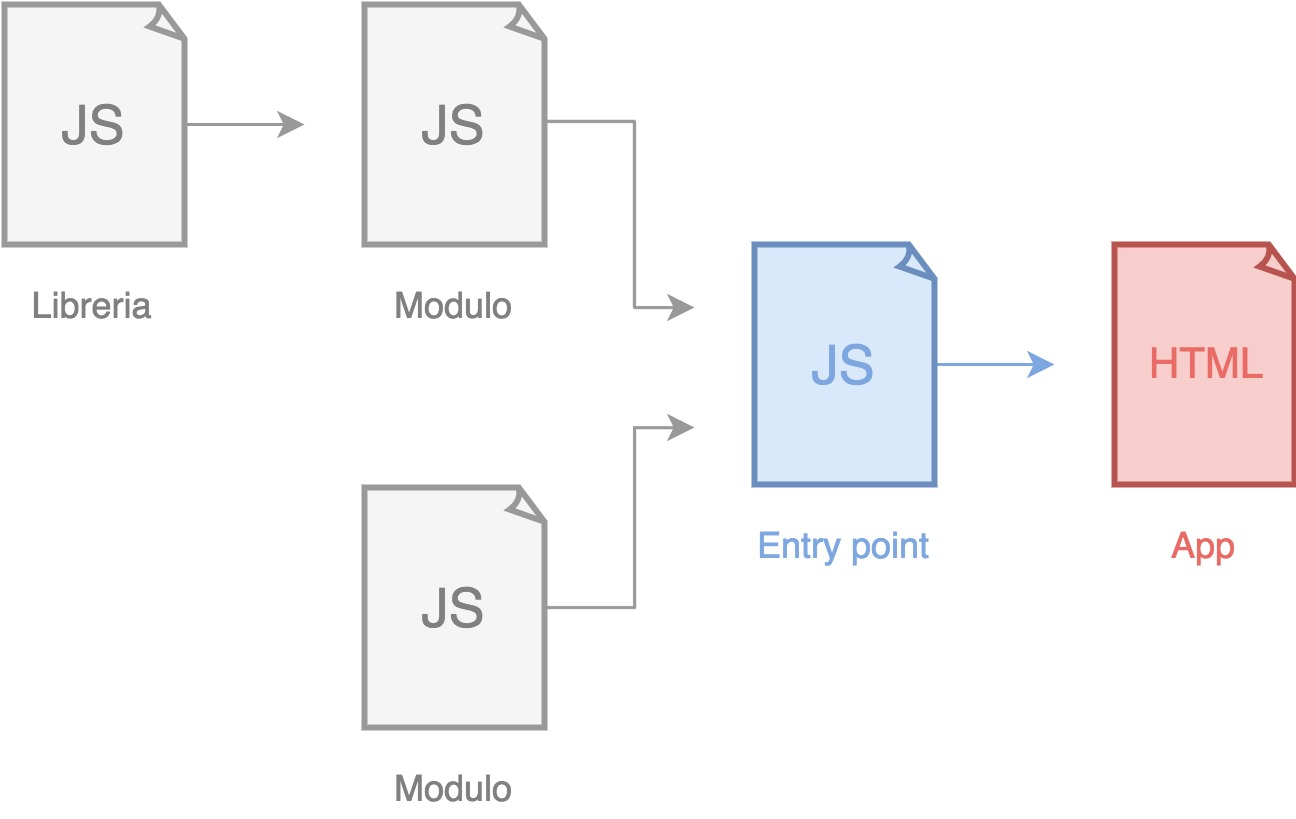
\includegraphics[width=9cm]{./images/webpackWorkflow}
\caption{Rappresentazione del sistema di impacchettamento di Webpack.}
\end{figure}

\subsection{Hot Module Replacement}
Un aspetto molto interessante di Webpack riguarda l'\textit{Hot Module Replacement} (HMR) che si occupa di aggiungere o rimuovere i pacchetti di dipendenze generati nel run-time dell'applicazione senza un aggiornamento completo della pagina. Questo è molto utile in fase di development in quanto consente di mantenere lo stato di una applicazione anche dopo aver effettuato modifiche al sorgente ed avere le nuove caratteristiche disponibili in maniera molto più veloce del normale aggiornando solo ciò che è necessario. 



\subsection{Tree Shaking}
La tecnica del \textit{Tree Shaking} permette di eliminare il codice inutilizzato all'interno della codebase. Quello che fa Webpack è andare ad analizzare a la struttura di \textit{Import} ed \textit{Export} del sorgente che, come abbiamo detto precedentemente nella sezione riguardante ES6, è statica ossia è possibile analizzarla a \textit{compile-time} senza la necessità di eseguire il codice. Una volta trovati gli elementi che non vengono utilizzati essi vengono classificati come “codice morto" e vengono marcati attraverso adeguati commenti. Webpack non si occupa di eliminare questi elementi ma affida il compito ad un eventuale \textit{Minifier} (come ad esempio \textit{UglifyJS}) che si occupa di ottimizzare il codice Javascript.

\section{React}
React è una libreria scritta da Facebook per la creazione di interfacce utente interattive in maniera funzionale ed altamente scalabile. Si basa sul concetto di "componente" come elemento base fondamentale, ossia un pezzo di interfaccia che ha uno stato proprio ed è riutilizzabile all'interno del servizio (codice \ref{exampleReactComponents}). Il concetto funzionale di composizione si adatta benissimo a React: un componente complesso dovrebbe essere formato da componenti più piccoli e agnostici che possono quindi essere riutilizzati in altri componenti complessi.

\begin{listing}[ht]
\inputminted{jsx}{sources/exampleReactComponents.js}
\caption{Esempio di composizione tra componenti React.}
\label{exampleReactComponents}
\end{listing}

Viene utilizzato in produzione sia da Facebook che da Instagram e fa uso di diverse tecnologie all'avanguardia come il \textit{Virtual DOM} ed il \textit{Server-side Rendering} \cite{WheelerOnReact}.

\subsection{Virtual DOM}
Il  \textit{Document Object Model} (DOM) è una API che definisce la struttura di un documento HTML e come essa viene acceduta e manipolata. E' una rappresentazione ad oggetti di una pagina web la quale può essere modificata con un linguaggio di scripting come Javascript.
Per fare un esempio pratico, lo standard DOM stabilisce che l'interfaccia \textit{Document} rappresenti l'intera pagina HTML e che concettualmente sia il nodo root. L'interfaccia \textit{Node} rappresenta invece l'elemento base ossia il singolo nodo all'interno di un documento e l'implementazione di questa richiede la creazione dei metodi per la gestione del nodo stesso e dei propri figli \cite{HWRWhatIsDOM}.

Quando parliamo di Virtual DOM parliamo di un'astrazione sopra l'astrazione del DOM. Modificare quest'ultimo non è particolarmente dispendioso (si tratta solamente di modificare un oggetto Javascript) è tuttavia il processo di lettura e di “ridisegno" della pagina da parte del browser il vero problema. Questa tecnologia riesce a risolvere il suddetto problema mantenendo in memoria una rappresentazione del DOM reale che utilizza il design pattern \textit{Observer}\footnotemark per capire quale particolare nodo è stato modificato generando successivamente un nuovo albero derivato dal precedente ma con il nuovo stato. A questo punto effettua complessi algoritmi di differenza per trovare il numero minimo di passaggi per aggiornare il DOM reale per poter infine effettuare la riconciliazione \cite{MishraOnVirtualDOM}.

Il concetto che permette al Virtual DOM di garantire prestazioni maggiori sul DOM reale consiste nell'aggiornamento aggregato. Tutti i cambiamenti effettuati da un evento (che sono i passaggi trovati dall'algoritmo di differenza) vengono aggregati ed il DOM viene ridisegnato solamente una volta.

\begin{figure}[h]
\centering 
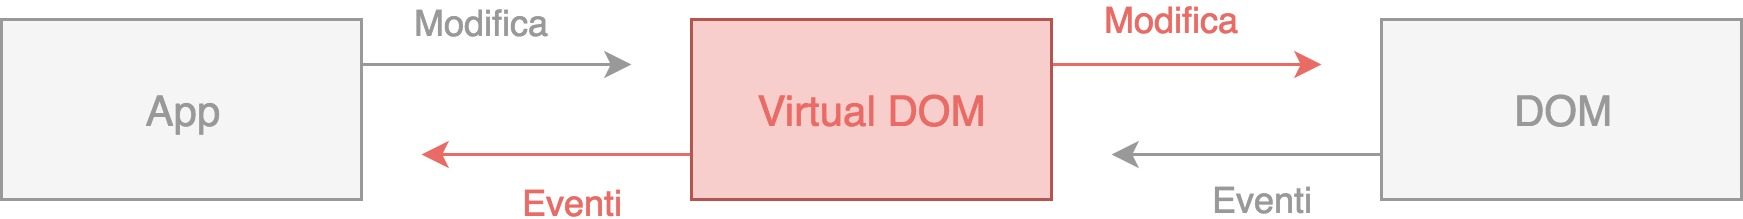
\includegraphics[width=13cm]{./images/virtualDOMWorkflow}
\caption{Posizione del Virtual DOM all'interno di una applicazione React.}
\end{figure}

React implementa il Virtual DOM attraverso \textit{JSX}, una estensione di ECMAScript simile ad XML che permette di scrivere elementi di markup con una sintassi simile all'HTML all'interno dei componenti dell'interfaccia. Portare l'HTML all'interno del codice sorgente Javascript offre dei vantaggi non banali come ad esempio il debugging compile-time degli errori di sintassi durante la costruzione del DOM, la versatilità di avere un linguaggio di scripting per effettuare composizione ed altre azioni dinamiche e sopratutto avere una perfetta separazione tra componenti differenti.

\footnotetext{Il design pattern Observer si struttura di un oggetto chiamato “Subject" che mantiene una lista di altri oggetti dipendenti chiamati "Observers" e li notifica ogni qualvolta il suo stato viene modificato.}

\subsection{Server-side rendering}
React è una libreria \textit{isomorfica}, è in grado di essere eseguita sia lato client che lato server traendo vantaggio da NodeJS ed il fatto che il principale linguaggio di programmazione per entrambi gli ambienti sia sempre Javascript.
Il vantaggio di eseguire React anche lato server risiede nella prima visualizzazione. In una Single Page Application normale durante il primo caricamento vengono scaricati gli elementi base per la sua esecuzione e successivamente viene eseguito il codice Javascript per il rendering del suo stato iniziale. La seconda fase può essere ulteriormente pesante, basti pensare che possono essere effettuate ulteriori richieste per soddisfare il normale fabbisogno dell'applicazione.

La tecnica del Server-side rendering permette di semplificare questa prima visualizzazione interpretando i componenti React lato server e restituendo una pagina iniziale con la Single Page Application già avviata e fornita di tutti i dati di cui avrebbe normalmente bisogno. Esistono tuttavia delle problematiche non proprio da sottovalutare: il fatto che in ogni caso l'utente non può comunque effettuare alcun tipo di interazione con l'applicazione finché React non viene scaricato anche dal client; che il primo \textit{TTFB (Time To First Byte)}\footnotemark è generalmente più lento del normale in quanto ci sono più computazioni lato server da effettuare per compilare il codice React; che le computazioni server-side potrebbero non essere veloci come quelle effettuate client-side causando un considerevole calo di prestazioni \cite{GrigoryanOnServerSideRendering}.

\footnotetext{Il Time To First Byte è solitamente utilizzato come misura di quanto veloce un server web risponde ad una richiesta, ed è in pratica la durata che intercorre tra la richiesta effettuata dall'utente e il primo byte di risposta del server \cite{GrahamOnTTFB}.}  
    
    \bibliographystyle{unsrtnat}
    \bibliography{all}
\end{document}